\subsection{Chaînes de texte}

\subsubsection{\CCpp}

\label{C_strings}
Les chaînes C normales sont terminées par un zéro (chaînes \ac{ASCIIZ}).

La raison pour laquelle le format des chaînes C est ce qu'il est (terminé par zéro)
est apparemment historique:
Dans [Dennis M. Ritchie, \emph{The Evolution of the Unix Time-sharing System}, (1979)]
nous lisons:

\begin{framed}
\begin{quotation}
A minor difference was that the unit of I/O was the word, not the byte, because the PDP-7 was a word-addressed
machine. In practice this meant merely that all programs dealing with character streams ignored null
characters, because null was used to pad a file to an even number of characters.
\end{quotation}
\end{framed}
Une différence mineure était que l'unité d'E/S était le mot, pas l'octet, car le PDP-7 était une machine
adressée par mot. En pratique, cela signifiait que tous les programmes ayant à faire
avec des flux de caractères ignoraient le caractère nul, car nul était utilisé pour compléter un fichier
ayant un nombre impair de caractères.

\myindex{Hiew}

Dans Hiew ou FAR Manager ces chaînes ressemblent à ceci:

\begin{lstlisting}[style=customc]
int main()
{
	printf ("Hello, world!\n");
};
\end{lstlisting}

\begin{figure}[H]
\centering
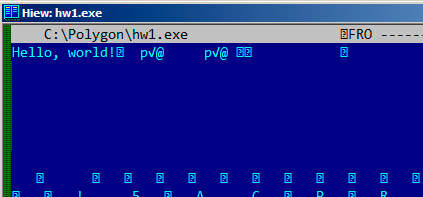
\includegraphics[width=0.8\textwidth]{digging_into_code/strings/C-string.png}
\caption{Hiew}
\end{figure}

% FIXME видно \n в конце, потом пробел

\subsubsection{Borland Delphi}
\myindex{Pascal}
\myindex{Borland Delphi}

Une chaîne en Pascal et en Delphi de Borland est précédée par sa longueur sur 8-bit
ou 32-bit.

Par exemple:

\begin{lstlisting}[caption=Delphi,style=customasmx86]
CODE:00518AC8                 dd 19h
CODE:00518ACC aLoading___Plea db 'Loading... , please wait.',0

...

CODE:00518AFC                 dd 10h
CODE:00518B00 aPreparingRun__ db 'Preparing run...',0
\end{lstlisting}

\subsubsection{Unicode}

\myindex{Unicode}

Souvent, ce qui est appelé Unicode est la méthode pour encoder des chaînes où chaque
caractère occupe 2 octets ou 16 bits.
Ceci est une erreur de terminologie répandue.
Unicode est un standard pour assigner un nombre à chaque caractère dans un des nombreux
systèmes d'écriture dans le monde, mais ne décrit pas la méthode d'encodage.

\myindex{UTF-8}
\myindex{UTF-16LE}
Les méthodes d'encodage les plus répandues sont: UTF-8 (est répandue sur Internet
et les systèmes *NIX) et UTF-16LE (est utilisé dans Windows).

\myparagraph{UTF-8}

\myindex{UTF-8}
UTF-8 est l'une des méthodes les plus efficace pour l'encodage des caractères.
Tous les symboles Latin sont encodés comme en ASCII, et les symboles après la table
ASCII sont encodés en utilisant quelques octets.
0 est encodé comme avant, donc toutes les fonctions C de chaîne standard fonctionnent
avec des chaînes UTF-8 comme avec tout autre chaîne.

Voyons comment les symboles de divers langages sont encodés en UTF-8 et de quoi ils
ont l'air en FAR, en utilisant la page de code 437\footnote{L'exemple et les traductions ont été pris d'ici:
\url{http://www.columbia.edu/~fdc/utf8/}}:

\begin{figure}[H]
\centering
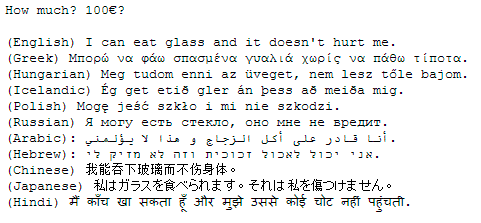
\includegraphics[width=0.8\textwidth]{digging_into_code/strings/multilang_sampler.png}
\end{figure}

% FIXME: cut it
\begin{figure}[H]
\centering
\myincludegraphics{digging_into_code/strings/multilang_sampler_UTF8.png}
\caption{FAR: UTF-8}
\end{figure}

Comme vous le voyez, la chaîne en anglais est la même qu'en ASCII.

Le hongrois utilise certains symboles Latin et des symboles avec des signes diacritiques.

Ces symboles sont encodés en utilisant plusieurs octets, qui sont soulignés en rouge.
C'est le même principe avec l'islandais et le polonais.

Il y a aussi le symbole de l'\q{Euro} au début, qui est encodé avec 3 octets.

Les autres systèmes d'écritures n'ont de point commun avec Latin.

Au moins en russe, arabe hébreux et hindi, nous pouvons voir des octets récurrents,
et ce n'est pas une surprise: tous les symboles d'un système d'écriture sont en général
situés dans la même table Unicode, donc leur code débute par le même nombre.

Au début, avant la chaîne \q{How much?}, nous voyons 3 octets, qui sont en fait le
\ac{BOM}. Le \ac{BOM} défini le système d'encodage à utiliser.

\myparagraph{UTF-16LE}

\myindex{UTF-16LE}
\myindex{Windows!Win32}
De nombreuses fonctions win32 de Windows ont le suffixes \TT{-A} et \TT{-W}.
Le premier type de fonctions fonctionne avec les chaînes normales, l'autre, avec
des chaîne UTF-16LE (\emph{large}).

Dans le second cas, chaque symbole est en général stocké dans une valeur 16-bit de
type \emph{short}.

Les symboles Latin dans les chaînes UTF-16 dans Hiew ou FAR semblent être séparés
avec un octet zéro:

\begin{lstlisting}[style=customc]
int wmain()
{
	wprintf (L"Hello, world!\n");
};
\end{lstlisting}

\begin{figure}[H]
\centering
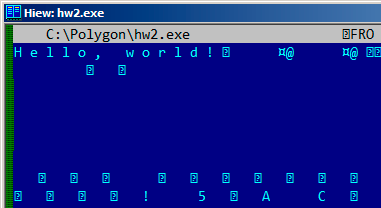
\includegraphics[width=0.8\textwidth]{digging_into_code/strings/UTF16-string.png}
\caption{Hiew}
\end{figure}

Nous voyons souvent ceci dans les fichiers système de \gls{Windows NT}:

\begin{figure}[H]
\centering
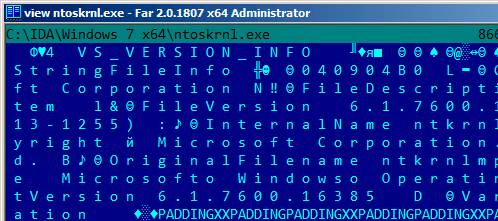
\includegraphics[width=0.8\textwidth]{digging_into_code/strings/ntoskrnl_UTF16.png}
\caption{Hiew}
\end{figure}

\myindex{IDA}
Les chaînes avec des caractères qui occupent exactement 2 octets sont appelées \q{Unicode}
dans \IDA:

\begin{lstlisting}[style=customasmx86]
.data:0040E000 aHelloWorld:
.data:0040E000                 unicode 0, <Hello, world!>
.data:0040E000                 dw 0Ah, 0
\end{lstlisting}

Voici comment une chaîne en russe est encodée en UTF-16LE:

\begin{figure}[H]
\centering
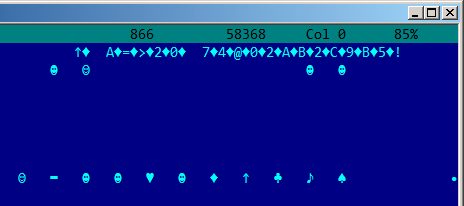
\includegraphics[width=0.8\textwidth]{digging_into_code/strings/russian_UTF16.png}
\caption{Hiew: UTF-16LE}
\end{figure}

Ce que nous remarquons facilement, c'est que les symboles sont intercalés par le
caractère diamant (qui a le code ASCII 4). En effet, les symboles cyrilliques sont
situés dans le quatrième plan Unicode.
Ainsi, tous les symboles cyrillique en UTF-16LE sont situés dans l'intervalle \TT{0x400-0x4FF}.

Retournons à l'exemple avec la chaîne écrite dans de multiple langages.
Voici à quoi elle ressemble en UTF-16LE.

% FIXME: cut it
\begin{figure}[H]
\centering
\myincludegraphics{digging_into_code/strings/multilang_sampler_UTF16.png}
\caption{FAR: UTF-16LE}
\end{figure}

Ici nous pouvons aussi voir le \ac{BOM} au début.
Tous les caractères Latin sont intercalés avec un octet à zéro.

Certains caractères avec signe diacritique (hongrois et islandais) sont aussi soulignés en rouge.

% subsection:
\subsubsection{Base64}
\myindex{Base64}

L'encodage base64 est très répandu dans les cas où vous devez transférer des données
binaires sous forme de chaîne de texte.

Pour l'essentiel, cet algorithme encode 3 octets binaires en 4 caractères imprimables:
toutes les 26 lettres Latin (à la fois minuscule et majuscule), chiffres, signe plus
(\q{+}) et signe slash (\q{/}), 64 caractères en tout.

Une particularité des chaînes base64 est qu'elles se terminent souvent (mais pas
toujours) par 1 ou 2 symbole égal (\q{=}) pour l'alignement, par exemple:

\begin{lstlisting}
AVjbbVSVfcUMu1xvjaMgjNtueRwBbxnyJw8dpGnLW8ZW8aKG3v4Y0icuQT+qEJAp9lAOuWs=
\end{lstlisting}

\begin{lstlisting}
WVjbbVSVfcUMu1xvjaMgjNtueRwBbxnyJw8dpGnLW8ZW8aKG3v4Y0icuQT+qEJAp9lAOuQ==
\end{lstlisting}

Le signe égal (\q{=}) ne se rencontre jamais au milieu des chaînes encodées en base64.

maintenant, un exemple d'encodage manuel.
Encodons les octets hexadécimaux 0x00, 0x11, 0x22, 0x33 en une chaîne base64:

\lstinputlisting{digging_into_code/strings/base64_ex.sh}

Mettons ces 4 octets au forme binaire, puis regroupons les dans des groupes de 6-bit:

\begin{lstlisting}
|  00  ||  11  ||  22  ||  33  ||      ||      |
00000000000100010010001000110011????????????????
| A  || B  || E  || i  || M  || w  || =  || =  |
\end{lstlisting}

Les trois premiers octets (0x00, 0x11, 0x22) peuvent être encodés dans 4 caractères
base64 (``ABEi''), mais le dernier (0x33) --- ne le peut pas, donc il est encodé
en utilisant deux caractères (``Mw'') et de symbole (``='') de padding est ajouté
deux fois pour compléter le dernier groupe à 4 caractères.
De ce fait, la longueur de toutes les chaînes en base64 correctes est toujours divisible
par 4.

\myindex{XML}
\myindex{PGP}
Base64 est souvent utilisé lorsque des données binaires doivent être stockées dans
du XML.  Les clefs PGP ``Armored'' (i.e., au format texte) et les signatures sont
encodées en utilisant base64.

Certains essayent d'utiliser base64 pour masquer des chaînes:
\url{http://blog.sec-consult.com/2016/01/deliberately-hidden-backdoor-account-in.html}%
\footnote{\url{http://archive.is/nDCas}}.

\myindex{base64scanner}
Il existe des utilitaires pour rechercher des chaînes base64 dans des fichiers binaires
arbitraires.
L'un d'entre eux est base64scanner\footnote{\url{https://github.com/DennisYurichev/base64scanner}}.

\myindex{UseNet}
\myindex{FidoNet}
\myindex{Uuencoding}
\myindex{Phrack}
Un autre système d'encodage qui était très répandu sur UseNet et FidoNet est l'Uuencoding.
Les fichiers binaires sont toujours encodés au format Uuencode dans le magazine Phrack.
Il offre à peu près la même fonctionnalité, mais il est différent de base64 dans
le sens où le nom de fichier est aussi stocké dans l'entête.

\myindex{Tor}
\myindex{base32}
À propos: base64 à un petit frère: base32, alphabet qui a ~10 chiffres et ~26 caractères Latin.
Un usage répandu est les adresses onion%
\footnote{\url{https://trac.torproject.org/projects/tor/wiki/doc/HiddenServiceNames}},
comme: \\
\url{http://3g2upl4pq6kufc4m.onion/}.
\ac{URL} ne peut pas avoir de mélange de casse de caractères Latin, donc, c'est apparemment
pourquoi les développeurs de Tor ont utilisé base32.



